
\documentclass[a4paper,USenglish,cleveref, autoref, thm-restate, anonymous]{lipics-v2021}
%This is a template for producing LIPIcs articles. 
%See lipics-v2021-authors-guidelines.pdf for further information.
%for A4 paper format use option "a4paper", for US-letter use option "letterpaper"
%for british hyphenation rules use option "UKenglish", for american hyphenation rules use option "USenglish"
%for section-numbered lemmas etc., use "numberwithinsect"
%for enabling cleveref support, use "cleveref"
%for enabling autoref support, use "autoref"
%for anonymousing the authors (e.g. for double-blind review), add "anonymous"
%for enabling thm-restate support, use "thm-restate"
%for enabling a two-column layout for the author/affilation part (only applicable for > 6 authors), use "authorcolumns"
%for producing a PDF according the PDF/A standard, add "pdfa"

\pdfoutput=1 %uncomment to ensure pdflatex processing (mandatatory e.g. to submit to arXiv)
\hideLIPIcs  %uncomment to remove references to LIPIcs series (logo, DOI, ...), e.g. when preparing a pre-final version to be uploaded to arXiv or another public repository

%\graphicspath{{./graphics/}}%helpful if your graphic files are in another directory

\bibliographystyle{plainurl}% the mandatory bibstyle

\title{Cross-Domain Integrity with Controller Labels and Endorsement}% mandatory

%\titlerunning{Dummy short title} %TODO optional, please use if title is longer than one line

\author{Isaac Sheff}{Heliax, Buffalo, USA \and \url{https://isaacsheff.com} }{isaac@heliax.dev}{https://orcid.org/0000-0002-1825-0097}{[(Optional) author-specific funding acknowledgements]}%TODO mandatory, please use full name; only 1 author per \author macro; first two parameters are mandatory, other parameters can be empty. Please provide at least the name of the affiliation and the country. The full address is optional. Use additional curly braces to indicate the correct name splitting when the last name consists of multiple name parts.

% \author{Christopher W. Goes}{Heliax, Berlin, Germany}{cwgoes@heliax.dev}{[orcid]}{[funding]}

\authorrunning{I. Sheff \& C. W. Goes} %TODO mandatory. First: Use abbreviated first/middle names. Second (only in severe cases): Use first author plus 'et al.'

\Copyright{Isaac Sheff and Christpher Goes} %TODO mandatory, please use full first names. LIPIcs license is "CC-BY";  http://creativecommons.org/licenses/by/3.0/

\ccsdesc[100]{\textcolor{red}{Replace ccsdesc macro with valid one}} %TODO mandatory: Please choose ACM 2012 classifications from https://dl.acm.org/ccs/ccs_flat.cfm 

\keywords{Dummy keyword} %TODO mandatory; please add comma-separated list of keywords

\category{} %optional, e.g. invited paper

\relatedversion{} %optional, e.g. full version hosted on arXiv, HAL, or other respository/website
%\relatedversiondetails[linktext={opt. text shown instead of the URL}, cite=DBLP:books/mk/GrayR93]{Classification (e.g. Full Version, Extended Version, Previous Version}{URL to related version} %linktext and cite are optional

%\supplement{}%optional, e.g. related research data, source code, ... hosted on a repository like zenodo, figshare, GitHub, ...
%\supplementdetails[linktext={opt. text shown instead of the URL}, cite=DBLP:books/mk/GrayR93, subcategory={Description, Subcategory}, swhid={Software Heritage Identifier}]{General Classification (e.g. Software, Dataset, Model, ...)}{URL to related version} %linktext, cite, and subcategory are optional

%\funding{(Optional) general funding statement \dots}%optional, to capture a funding statement, which applies to all authors. Please enter author specific funding statements as fifth argument of the \author macro.

\acknowledgements{}%optional

%\nolinenumbers %uncomment to disable line numbering



%Editor-only macros:: begin (do not touch as author)%%%%%%%%%%%%%%%%%%%%%%%%%%%%%%%%%%
% \EventEditors{John Q. Open and Joan R. Access}
% \EventNoEds{2}
% \EventLongTitle{42nd Conference on Very Important Topics (CVIT 2016)}
% \EventShortTitle{CVIT 2016}
% \EventAcronym{CVIT}
% \EventYear{2016}
% \EventDate{December 24--27, 2016}
% \EventLocation{Little Whinging, United Kingdom}
% \EventLogo{}
% \SeriesVolume{42}
% \ArticleNo{23}
%%%%%%%%%%%%%%%%%%%%%%%%%%%%%%%%%%%%%%%%%%%%%%%%%%%%%%


% Non-template imports
\usepackage{tikz}

% Non-template MACROS
\newcommand{\N}{\mathbb{N}}
\newcommand{\abs}[1]{\left|{#1}\right|}
\newcommand{\p}[1]{{\ensuremath{\left({{#1}}\right)}}}
\newcommand{\cb}[1]{{\left\{{{#1}}\right\}}}
\newcommand{\sqb}[1]{{\left[{{#1}}\right]}}
\newcommand{\an}[1]{{\left\langle{{#1}}\right\rangle}}
\newcommand{\ceil}[1]{{\ensuremath{\left\lceil{{#1}}\right\rceil}}}
\newcommand{\bb}[1]{{\left\llbracket{{#1}}\right\rrbracket}}
\newcommand{\tb}[1]{{\textrm{\textbf{{#1}}}}}
\newcommand{\ti}[1]{{\emph{{#1}}}}
\newcommand{\tallpipe}[2]{%
  {%
    \ensuremath{%
      \begin{array}{@{}r|l@{}}%
        {{#1}}&{{#2}}%
      \end{array}%
    }%
  }%
}
\newcommand{\join}{\mathbin{\sqcup}}
\newcommand{\meet}{{\ensuremath{\sqcap}}}
\newcommand{\eqdef}{\ensuremath{\overset{\mathrm{def}}{=}}}

\newcommand{\resources}{{\ensuremath{\mathcal R}}}


\newcommand{\colort}[2]{{\color{#1}{#2}}}
\newcommand{\red}[1]{\colort{red}{#1}}
\newcommand{\blue}[1]{\colort{blue}{#1}}
\newcommand{\green}[1]{{\colort{DarkGreen}{#1}}}
\newcommand{\purple}[1]{{\colort{purple}{#1}}}
\newcommand{\orange}[1]{{\colort{orange}{#1}}}
\newcommand{\gray}[1]{{\colort{gray}{#1}}}

\newcommand{\basecoin}{\blue{BaseCoin}}
\newcommand{\basechain}{\blue{BaseChain}}
\newcommand{\sidechain}{\purple{SideChain}}

\newcommand{\JuvixCore}{\ensuremath{\mathsf{JuvixCore}}}
\newcommand{\Geb}{\ensuremath{\mathsf{Geb}\,}}
\newcommand{\Juvix}{\ensuremath{\mathsf{Juvix}}}
\newcommand{\VampIR}{\ensuremath{\mathsf{VampIR}}}
\newcommand{\LambdaIR}{\ensuremath{\mathsf{Lambda}}}




\begin{document}

\maketitle

%TODO mandatory: add short abstract of the document
\begin{abstract}
In distributed systems, mutable digital objects typically require some state machine to decide on their definitive current state.
This state machine can be replicated to enhance availability and fault tolerance.
We call the authoritative state machine of a digital object its \emph{controller}.
Typical examples of controllers defining objects include a database storing a record, or a blockchain storing the current state of a smart contract.
Without some kind of controller, different parties may have contradictory notions of what the state is, and no way to reconcile them.
In a distributed system, some controllers may be \emph{byzantine}, and make duplicitous or incoherent statements about state. 

Here we design rules and procedures for a multi-state-machine ecosystem, featuring digital objects, or \emph{resources}, with application-defined state-dependent rules for how they can be updated. 
Resources can even be \emph{shielded}, where the and state of the resource is hidden from the controller itself. 
Each controller can express an authoritative state, including authoritative resource states. 
Each resource is also labeled with a controller identifier, whose state is definitive for this resource. 
Resources can transfer between controllers, and updates can depend on the state of other resources maintained by other controllers, so resource labels also express a \emph{dependency graph} detailing which controllers, if they were byzantine, may have corrupted this resource.
In a sense, these labels represent a distributed \emph{taint tracking} or \emph{dynamic information flow control} solution.
One challenge is avoiding size explosion in this dependency graph: we enable removing unnecessary parts of history when, say, a resource transfers from $A$ to $B$ and back to $A$ again.
In taint tracking or information flow control terms, these operations require \emph{endorsement}.
Our resource controller operations generalize a number of techniques used in blockchain settings.
We define rules and procedures for creating, updating, transferring, and tracking the state of labeled resources, and prove that our rules maintain safety properties including \emph{causal resource history} and \emph{consistent controller labels}.
We also prove that some operations (non-blocking local reduction) are impossible without violating these safety properties. 
\end{abstract}

\section{Introduction}
Distributed platform interoperability is crucial to improve cost, usability, adoption, and even security. 
When When applications must share a state machine (or, more generally, \emph{controller}) to interact, there is an incentive to push all applications onto one controller trustworthy enough (and with enough throughput) for everyone. 
Attempts to create such a controller typically require trust in a single authority (e.g. AWS\cite{citation-needed}) or an extremely expensive global consensus (e.g., Ethereum) and remain inadequate for some applications:
 JP~Morgan does not trust Ethereum to control their accounts~\cite{onyx}.
In fact, it is unlikely that \emph{all} worthwhile applications will ever agree on a controller who can manage all of their state.
This is why interoperability is so important: the internet works not because we all trust some single authority to manage all of it but because many different applications in different trust domains can interact. 

Nevertheless, cross-domain data integrity remains a challenge.
While  existing systems can track controllers that may have affected each datum~\cite{dista,fabric}, these can easily lead to a state explosion: each object's label features an ever-growing set of controllers that may have affected it. 
In blockchain ecosystems, some protocols cleverly get around this: objects can reduce their labeling burden when one controller \emph{endorses} another, reviewing (some part of) its history and, crucially, pledging not to endorse a contradictory history.
For example, blockchains can create \emph{wrapped} tokens with IBC and ICS20~\cite{wrapped,ibc, ics20}. 
A wrapper represents a controller that had previously controlled the token, and nested wrappers represent a list of controllers. 
A controller can \emph{unwrap} a token with a simple but effective review of the wrapped token history. 
It checks a crucial invariant: it will unwrap no more tokens of each type from each destination than it wrapped. 
In this work, we generalize this controller history tracking and endorsement approach, and enable fully general transferable digital objects (not only tokens), with arbitrary transactions. 
Crucially, this means generalizing resource histories from a list of wrapping controllers to a DAG.
This endorsement approach differs somewhat from some Information Flow Control approaches~\cite{fabric, citation-needed}, in that we assume controllers can review and endorse entire execution traces of other controllers, and check for contradictions.

Here, we introduce a novel protocol for controllers that enables very general operations across state machines with different trust domains.
Our controller protocol will eventually be part of a larger unified multi-state-machine architecture, with standards for each state machine, as well as transferable objects called \emph{resources}~\cite{resource}.
Here, we detail controller operations that allow our architecture to generalize many existing techniques (including many cross-chain and side-chain operations). 




% ICS: an example, which IBC can handle:
% Suppose Alice wants to move some {\basecoin}s from \basechain\ to \sidechain, use them for some transactions involving other currencies and digital objects from other chains, and then move her remaining {\basecoin}s back to {\basechain}.
% In controller terms, \basechain\ is a state machine that determines the definitive state of Alice's {\basecoin}s: \basechain\ is the controller for each \basecoin\ digital object. 
% Alice wants to change her {\basecoin}s' controller to be \sidechain, and then do some transactions using them and other \sidechain-controlled objects. 
% Controllers can fail (they can fork, and enable double-spends), so in some sense, her {\basecoin}s will only be as trustworthy as \sidechain: if \sidechain\ has forked, no one should trust any statements \sidechain\  makes about the definitive state of Alice's {\basecoin}s.
% Alice then wants to take her \sidechain-controlled {\basecoin}s, and change their controller back to \basechain.
% She may even then want to ``remove'' \sidechain\ from her {\basecoin}s' histories.
% If \basechain\ reviews \sidechain's history, it may be able to ``endorse'' everything it has done, establishing that whatever has happened to Alice's {\basecoin}s ``may as well have happened'' on \basechain, so Alice's {\basecoin}s are not forever ``tainted'' by {\sidechain}.
% This is important if \sidechain\ should later prove unreliable. 
% TODO: diagram this

\subsection{Controllers}  
Controllers are a key component of any transaction processing state machine, including blockchains~\cite{smr,statemachine}.
We define the controller as the component that \emph{orders}: it decides on an ever-growing sequence of transactions defining the execution trace, and thus the current state, of a state machine.
% ICS: for the DISC audience, this is unnecessary: For some blockchains, this sequence is literally the blockchain data structure.
%If the \textit{global state machine} \replace{includes}{covers/treats/...} all resources, commitments, and nullifiers ever produced, then each controller decides an order for transactions that use its portion of the state machine:\footnote{is it really a portion of \emph{the state machine}, as opposed to just state?} those using its own portion of the state.
Controllers do not necessarily compute and store this state themselves, although it may be efficient to do so.
Committing to an ever-growing sequence of transactions, however, does require that controllers keep \textit{some} state, to ensure they do not \emph{fork}: commit two contradictory traces (neither is a prefix of the other).
Forks are the essence of, for example, double-spend attacks~\cite{Abraham2017}.

Trusting controllers is fundamental for digital objects: tables in Postgres maintain their invariants iff the database is working properly~\cite{citation-needed}.
Similarly, a smart contract on Ethereum is consistent iff the Ethereum controller is working properly\cite{citation-needed?}.
We categorize controllers in terms of safety and liveness:
\begin{itemize}
\item \emph{Safe} controllers commit transactions only in a totally ordered sequence (called a \emph{trace}): they do not fork.
The \emph{state} of a valid controller is unique and defined as the result serially applying the transactions (atomic transitions defined by the state machine) in the trace committed, and ignoring any \emph{invalid} transactions (as defined by the state machine).
  \emph{Unsafe} controllers are also called \emph{malicious} or \emph{Byzantine}.  
\item \emph{Live} controllers eventually respond to valid queries, and append valid transactions to their trace.
  Controllers that are not live are called \emph{unlive}, \emph{crash-prone}, or sometimes just \emph{crashed}.
\end{itemize}
In general, we assume all unsafe controllers are unlive: controllers that are not following the specification could just choose to ignore all queries.


\subsection{Resources}
Our architecture tracks specific types of transferable digital objects, which we call \emph{resources}~\cite{resource}.
We can encode extremely general mutable state with resources, but resources themselves are fairly simple.
Each resource can be \emph{not yet created}, \emph{created}, or \emph{consumed}.
Resources are \emph{not yet created} by default, can transition to \emph{created}, and then to \emph{consumed}.
Resources transition between these states in transactions ordered by controllers.
Each resource therefore specifies a single controller that can order transactions for each type of transition, ensuring there is a single authority in charge of deciding whether each transition has or has not occurred.
Transactions which perform a state transition but are ordered by the wrong controller are \emph{invalid}.

Each controller's state carries cryptographic accumulators (e.g. Merkle roots~\cite{citation-needed}) representing the set of resources created by transactions ordered by this controller and the set of resources consumed.
If a resource is neither created nor consumed, it is \emph{not yet created}.
Resources can have complex proof obligations (which we call \emph{resource logics}) determining when they can be created or consumed, and these may depend on the state of other resources. % ICS: eliding for now: , even on other controllers.
A resource logic can for example, specify exactly what programs can consume this resource: it would require a proof that the resources created are precisely the outputs of running a particular program with the consumed resources as inputs.
Such a proof might be as simple as a full execution trace of the program, or as complex as a zero-knowledge proof~\cite{citation-needed}.
Through these logics, resources can encode fairly arbitrary state, not limited to scalar registers or tokens, while still allowing ZKP-style confidential transactions~\cite{resource}.

\subsection{Transactions}
Transactions are atomic state transitions~\cite{smr,statemachine}.
For our purposes, transactions designate a set of resources (which must be \emph{created}) as \emph{inputs}, \emph{consume} some subset of their inputs, and \emph{create} some \emph{output} resources.
In general, we assume these transactions are deterministic, so each new state is uniquely defined.
Transactions can only update state controlled by one controller, and must include checkable proofs that all of the resource logics of each resource created or consumed are satisfied.
However, input resources may have been \emph{created} in a transaction on another controller.
Therefore, controllers can sync with one another, allowing transactions to check if resources on other controllers have been created.
These updates can be asynchronous, so it is possible a transaction will not immediately be able to prove that a resource has been created.

\subsection{Labels}
Resources themselves carry \emph{labels} concerning controllers who can or have affected the history (or ancestry) of that resource.
We will detail exactly what these labels will be later, but they include, among other things,
 a \emph{creating} controller, whose state defines whether this resource has transitioned from \emph{not yet created} to \emph{created}, and a \emph{terminal} controller, whose state defines whether this resource is \emph{consumed}.
Any transaction with this resource as an input must be ordered by its terminal controller.
This ensures there are never two controllers trying to consume the same resource with different transactions.
For example, imagine a resource representing a token, created on some controller $A$.
If controller $B$ orders a transaction that consumes this token and creates a new token called \emph{Alice}, and controller $C$ orders a transaction that consumes this token and creates a new token called \emph{Bob}, then we have a ``double-consume:'' together, \emph{Alice} and \emph{Bob}'s histories represent the token being consumed twice, which should not happen.
This is clearly a problem if the tokens have, say, monetary value: it's a double-spend~\cite{citation-needed}.
Terminal controllers solve the problem: if the resource specifies it can only be used by transactions on $B$, then the token can only be double-spent if $B$ forks.

We might imagine labels which include a set of \textit{affecting} controllers, who have influenced this resource's history (or provenance).
In general, we can ``transfer'' a resource from one controller to another: we consume a resource with one terminal controller, and produce a similar resource with a different terminal controller, and the old resource's terminal controller in its affecting controllers (encoded in its label). 

\subsection{Salad Example}
\begin{figure}
    \centering
    \includegraphics[width=\linewidth]{figs/salad_timeline.pdf}
    \caption{Timelines for 4 controllers, and resources for a virtual cooking application. Controllers are labeled with letters, and resources are labeled with numbers.}
    \label{fig:salad}
\end{figure}
Suppose four controllers ($A,B,C,$ and $D$) order transactions for a virtual cooking application (shown in~\cref{fig:salad}).
In the beginning, a tomato resource (0) and a cucumber resource (3) are on controller $A$.
The tomato resource transfers to $B$ (resource 0 is consumed, requiring whatever proofs are required to move a tomato, and resource 1 is created), and then, after some $B$-only transactions, it transfers to $D$ (resource 4).
Likewise, the cucumber resource transfers to $C$ and then to $D$ (resource 7).
On $D$, a transaction consumes both the tomato and cucumber resources to create a salad resource (resource 8). 
At this point, the salad resource's history depends on $A$, $B$, $C$, and $D$.
These are the affecting controllers of the salad's label.
If any of these controllers have been unsafe (as in~\cref{fig:saladfork}), there may be other resources elsewhere, claiming to represent the same tomato or cucumber that are supposedly part of this salad. 
The salad then transfers from $D$ to $A$, where the tomato and cucumber began.
Eventually, we want to allow $A$ to \emph{endorse} the salad's history, pledging not to endorse any alternative histories in which the cucumber or tomato did anything else, and removing the need to remember that $B$, $C$, or $D$ could have ``tainted'' the salad's history~\cite{dista}. 
They can be removed from the affecting controllers of the salad's label.

\section{Desiderata}
There are several properties we want our controllers and resource labels to have.
As a running example, consider~\cref{fig:saladfork}, a version of our salad example in which controller $B$ has forked into two traces: gray and black. 
Resource 10 (and therefore 11) has a \emph{conflicting} history with resource 2 (and therefore, 4, 8, and 9).


\subsection{Causal Resource History (CRH)}
We begin with a weak but relatively simple to maintain property: causally consistent resource history, or \emph{Causal Resource History (CRH)}~\cite{causal}.
A resource with CRH was created in a valid\footnote{\cite{resource} defines a ``valid'' transaction as not using an input that's already been consumed.
Here, as we lack global time, we require only that a transaction's inputs have not been consumed by a transaction in its \textit{causal} past.}
transaction, whose inputs were resources with CRH. 
This property is relatively easy to prove with recursive zero knowledge proofs (compared with some stricter properties we'll get to later)~\cite{nova}.
In general, in order to maintain CRH, a resource should carry a (recursive) proof that it was created in a valid transaction, the inputs of which had CRH proofs. 
In fact, CRH can be implemented in resource logics.

This property is not perfect: it still permits histories we might want to call \emph{inconsistent}, including double-consumes.
For example, in~\cref{fig:saladfork}, any future resource that depends on resources 9 and 11 (so, something constructed by consuming the salad and the tomato), would have a history in which the same tomato (which started as resource 0), is consumed twice, but would still have CRH.



\begin{figure*}
    \centering
    \centerline{
    \includegraphics[width=0.85\linewidth]{figs/salad_timeline_fork.pdf}
    }
    \caption{Controller $B$ has forked into two timelines (gray and black).
             Resources 10 and 11 \emph{conflict} with resources 2, 4, 8, and 9.}
    \label{fig:saladfork}
\end{figure*}

\subsection{Serializable Resource History (SRH)}
Here we define what we consider \emph{consistent}: each resource (individually) reflects some fully serializable history featuring only correct atomic transactions (and no forks)~\cite{serializability}. 
Equivalently, in the resource's history, all transactions are valid, and no resource is used as an input for a transaction after it has been consumed. 
In our~\cref{fig:saladfork} example, resources 11 and 9 individually have SRH, but they cannot both appear in the history of any future resource with SRH (no one can consume both as an input in some transaction).
Alternatively, you could not combine money from both sides of the double-spend for one big purchase.
SRH can be easily generalized to a group of resources by imagining a new resource that depends on all of the resources in the group, and checking if it has SRH.

Maintaining SRH requires some kind of mechanism for checking if two resources can both be part of some future resource's history. 
Effectively, any such mechanism checks for forks, and can be used to filter for resources that have SRH.

%If a resource is part of\footnote{\emph{is part of} in what sense part of ???} a consistent controller state, then it must have a consistent resource history. 
%Likewise, if some resource's ancestors include all the resources on a controller, and that resource has a consistent resource history, then that controller has a consistent controller state.\footnote{something to understand about \emph{controller state}, best with an example of some specific paradigmatic type of controller state}

In~\cref{sec:resourcevectorclocks}, we detail a technique for maintaining SRH for all resources, but it can require very expensive computation and requires each resource to carry an ever-growing set of controllers in its label. 
Instead, we allow users to introduce a little trust into the system, and dramatically improve day-to-day operations.
We will detail techniques for checking SRH while using our technique, but each check can require a lot of information.

\subsection{Consistent Controller Label (CCL)}
In general, a safe controller never uses a resource as a transaction input after it has been consumed: all inputs to any transaction it commits are created, unconsumed resources, and the transaction consumes (some subset of) those inputs, and creates new resources. 
The \emph{Consistent Controller Labels}  property (CCL) requires that if some resource~$r$ does not have SRH, then it has an unsafe controller in the \textit{affecting controllers} set in its label.
With CCL and CRH, if a user \textit{trusts} that a resource's affecting controllers are all safe, they can be sure the resource has a consistent resource history. 

% TODO: make this a little theorem and make a proof?

One easy way to maintain this would be to start with a system that maintains CRH, and label every resource with every controller involved in its history (affecting controllers). 
If all the controllers are safe, then the resource has SRH. 
For example, in~\cref{fig:saladfork}, resource 8's affecting controllers include $A$, $B$, $C$, and $D$.
However, we explore optimizations that allow removing unnecessary controllers from the affecting controllers set.
For instance, in~\cref{fig:saladfork}, $A$ can \emph{endorse} the history of resource 9, and remove $B$, $C$, and $D$ from its affecting controllers.
The key in this case is to ensure that any future resource that depends on both resource 9 and resource 11 \emph{will} include $B$ in its affecting controllers.
To accomplish this, we prevent $A$ from endorsing (and thus removing $B$ from) the history of both resource 9 and resource 11.

In~\cref{sec:consistentcontrollerstate}, we introduce Consistent Controller State, an even stronger property than SRH, along with a technique to maintain it, but we believe the inherent ``forks split the world'' drawbacks  make consistent controller state too strong to be worth using.

\section{Controller DAGs with Endorsement: a Technique for CCL}
\label{sec:dagswithendorsement}
In this approach, we maintain CRH and CCL, with relatively little overhead.
% ICS: we don't really define what little overhead means here.
% It's easiest to see what we're talking about there in contrast to other techniques (now in the appendix)
% The problem is that presenting all those other techniques first takes space and time. 
Resource label size can be kept proportional to the number of controllers in its history (in the worst case), but in the best case is much smaller.
Moving a resource between controllers is relatively cheap, requiring only few simple checks and a single endorsement (which can be done as two recursive ZKP checks).
Endorsements are not resource-specific, so they can be done opportunistically and their costs amortized. 

\subsection{Controller State}
Suppose that each controller has a unique \emph{controller id}.
Suppose also that each controller's entire state (including accumulators for which resources it has created and consumed, and everything else) can be uniquely identified with a digest or hash called a \emph{state root}.
We have a notion of one state (or state root) being provably \emph{after} another state (or state root) if the ``later'' one is the result of a (possibly empty) sequence of valid state transitions (transactions) ordered by the state root's controller, starting with the ``earlier'' one. 
We can define provably \emph{before} similarly. 

\noindent Each controller's state includes (but is not limited to) the
data in~\Cref{tab:controllerstate}.

\begin{table*}
\centerline{
\begin{tabular}{|l|l|p{0.5\textwidth}|}\hline
\textbf{Field} & \textbf{Type} & \textbf{Description} \\\hline
halted & boolean & Is this a halting state? There are no valid transitions from halting states.\\\hline
endorsement & map: controller id $\rightarrow$ state root & state roots of other controllers this controller has (non-recursively) endorsed.\\\hline
\end{tabular}}
\caption{Fields in a controller's state.}
\label{tab:controllerstate}
\end{table*}

\noindent The \textit{endorsement} map starts with every controller id mapping to genesis (whatever state root it must start with; this may be defined in the controller id itself).
There is one exception: the element for this controller's id is the state root for this state.
We also introduce a new type of transaction.
A controller id's endorsement element can be updated, given:
\begin{itemize}
    \item a proof that the new state root is provably after the old state root, and
    \item a proof that if the endorsed state root contains an endorsement for this controller, it endorsed a state root provably before this state (you can't endorse someone who has endorsed a fork of yourself).
\end{itemize}
Note that this update does \emph{not} require any kind of recursive update of controllers the endorsed controller has endorsed.

\subsection{Resource Controller Labels}
Each resource label includes a DAG representing controllers who have affected
the history of this resource. Each \textit{node} of this DAG includes the fields
in~\Cref{tab:resourcelabel}.
The set of all controllers from all the nodes of this DAG are the resource's \emph{affecting controllers}.


\begin{table*}
\centerline{
\begin{tabular}{|l|l|p{0.55\textwidth}|}\hline
\textbf{Field} & \textbf{Type} & \textbf{Description} \\\hline
controller & controller id & a controller who affected this resource's history \\\hline
state & state root & a state root from this controller \textit{after} (or equal to) the state resulting form the transaction that affected this resource's history \\\hline
removable & boolean & If this resource (or some part of its history) the result of a transaction that could \textit{only} have run on this controller, or would not be able to run on arbitrary controllers, then this must be false.\\\hline
reducing & $\bot$ or $\an{\textrm{controller id, state root}}$ & Are we in the process or removing this node from this controller DAG? (described below)\\\hline
\end{tabular}}
\caption{Fields in a resource controller label.}
\label{tab:resourcelabel}
\end{table*}

\noindent There must be exactly one sink of a controller DAG, which we call the resource's \textit{terminal node}.
The controller with the id specified in the terminal node is the resource's \textit{terminal} controller.
When discussing our~\cref{fig:saladfork} example, we write nodes as, for example, $A@11$, to denote controller $A$ with the state root it had just after creating resource 11.

\noindent In addition, each resource label includes the fields
in~\Cref{tab:resourcelabel2}.

\begin{table*}
\centerline{
\begin{tabular}{|l|l|p{0.5\textwidth}|}\hline
\textbf{Field} & \textbf{Type} & \textbf{Description} \\\hline
creating & node & specifies a particular node (not necessarily the terminal one) in the controller DAG which represents the creation of this resource.
The state corresponding to the state root of this node must prove this resource has been \emph{created}.\\\hline
backup & list of controller ids & If the terminal controller halts, who will be the new terminal controller? If that controller has halted, who will be the new terminal controller? and so on\dots\\\hline
\end{tabular}}
\caption{Fields in a resource label.}
\label{tab:resourcelabel2}
\end{table*}


\subsection{Creating a resource}
A transaction must use as inputs resources with the same terminal controller: the controller that orders the transaction. 
The terminal controller's state determines if any of the input resources have been consumed (which would make the transaction invalid).
To determine if all the input resources have in fact been created, one must check whether the creating controller of the resource has created it. 
To ensure CRH, we require the endorsement entry for each of the input resource's creating controllers to be provably after the state root for each resource's creating node. 
Since endorsement entries require valid proofs, this ensures CRH: each input resource is the result of a valid transaction whose inputs had CRH. 

A created resource can \textit{depend} on input resources, meaning the new resource's history includes those input resources, and their histories. 
In general, it is safe for a created resource to depend on all the input resources used in proofs of the resource's logic; this would work for very general applications.
However, we might allow resource logics to specify a subset of the input resources on which they depend. 
We might imagine a UTXO-style currency application~\cite{citation-needed} which tracks only input resources of the same currency as dependencies: anything which was necessary to authorize a ``spend'' isn't considered part of the history of the currency resource.

For any created resource, the controller DAG is the union of the controller DAGs of the input resources on which it depends, with an edge from their terminal controllers to a node featuring this controller's id and current state root. 
This node is the resource's \textit{creating} node. 
The controller node's \textit{removable} field should be false iff this transaction cannot be run on an arbitrary controller, but requires something special about this controller (e.g. issuing a currency, or a state change corresponding to a real-world action that can only be certified here). 
The controller may then include an additional edge from the creating node to a new terminal node, featuring a different controller id and a genesis state root. 

When the creating node is not the terminal node, this is a \textit{transfer}.
The resource has ``transferred'' to a different controller from its ancestors. 

For example, in~\cref{fig:saladfork}, resource 3 would need a creating node $A@3$ (representing the state controller $A$ had just after creating resource $3$).
Since $3$ is a transfer (it must be consumed on controller $C$), it also has terminal node $C@\bot$ ($\bot$ representing a genesis state root). 
Resource 3's controller DAG must, therefore, be (at least) $A@3 \rightarrow C@\bot$.

\subsection{Reducing a Controller DAG}
There are several ways to ``remove'' a node from a controller DAG.
These operations are transactions that consume the resource and replace it with a similar resource whose controller DAG is similar but missing one node. 
The simplest is condensing a single controller.

\subsubsection{Condensing a Single Controller}
If there is some subset of nodes featuring all the same controller id, and if it would not create a cycle, the subset can be replaced with a single node featuring the same controller id and a state root that is proven after (or equal to) all the state roots in the subset. 
All ancestors of any subset element become ancestors of the new node, and all descendants of the subset become descendants of the new node. 
This transition trivially preserves CCL, since it doesn't change the set of affecting controllers. 
It may be convenient to do this while creating a resource for simplicity.

For example, in~\cref{fig:saladfork}, suppose resource 3 has controller DAG $A@3 \rightarrow C@\bot$, so resource 6 could have controller DAG: $A@3 \rightarrow C@\bot\rightarrow C@5\rightarrow C@6$, but we can condense the $C$ nodes to reduce the controller DAG to: $A@3 \rightarrow C@6$.
Using the same process, we can reduce resource 9's controller DAG

\begin{center}
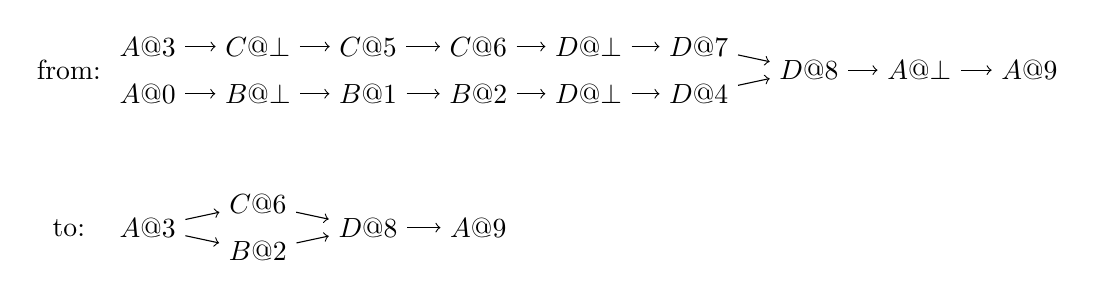
\begin{tikzpicture}
\node (from) at (0,2) {from:};
%% nodes
\node (FA3) at (1,2.3) {$A@3$};
\node (FCb) at (2.4,2.3) {$C@\bot$};
\node (FC5) at (3.8,2.3) {$C@5$};
\node (FC6) at (5.2,2.3) {$C@6$};
\node (FDb) at (6.6,2.3) {$D@\bot$};
\node (FD7) at (8,2.3) {$D@7$};
\node (FA0) at (1,1.7) {$A@0$};
\node (FBb) at (2.4,1.7) {$B@\bot$};
\node (FB1) at (3.8,1.7) {$B@1$};
\node (FB2) at (5.2,1.7) {$B@2$};
\node (FDb2) at (6.6,1.7) {$D@\bot$};
\node (FD4) at (8,1.7) {$D@4$};
\node (FD8) at (9.4,2) {$D@8$};
\node (FAb) at (10.8,2) {$A@\bot$};
\node (FA9) at (12.2,2) {$A@9$};
%%% edges
\draw[->] (FA3) -- (FCb);
\draw[->] (FCb) -- (FC5);
\draw[->] (FC5) -- (FC6);
\draw[->] (FC6) -- (FDb);
\draw[->] (FDb) -- (FD7);
\draw[->] (FA0) -- (FBb);
\draw[->] (FBb) -- (FB1);
\draw[->] (FB1) -- (FB2);
\draw[->] (FB2) -- (FDb2);
\draw[->] (FDb2) -- (FD4);
\draw[->] (FD7) -- (FD8);
\draw[->] (FD4) -- (FD8);
\draw[->] (FD8) -- (FAb);
\draw[->] (FAb) -- (FA9);

\node(to) at (0,0) {to:};
%% nodes
\node (A) at (1,0) {$A@3$};
\node (C) at (2.4,0.3) {$C@6$};
\node (B) at (2.4,-0.3) {$B@2$};
\node (D) at (3.8,0) {$D@8$};
\node (A9) at (5.2,0) {$A@9$};
%%% edges
\draw[->] (A) -- (C);
\draw[->] (A) -- (B);
\draw[->] (B) -- (D);
\draw[->] (C) -- (D);
\draw[->] (D) -- (A9);
\end{tikzpicture}
\end{center}

\subsubsection{Endorsement}
We can use the controller's endorsement map to remove unnecessary elements from a resource's controller DAG.
The idea is that if a resource's history involves moving to some intermediate controller, doing some transactions, and then moving on, the intermediate controller is \textit{arbitrary}: as long as other controllers are willing to check the part of the history done on the intermediate controller, they can claim they ``may as well have'' done those state changes themselves, and remove the intermediate controller.
This kind of endorsement-based DAG reduction generalizes IBC and ICS20's \emph{unwrapping} \cite{wrapped,ibc,ics20}.
In our~\cref{fig:saladfork} example, $A$ could endorse $C$, $D$, and (one fork of) $B$, and then reduce resource 9's controller DAG to just $A@9$.
The challenge is to do this in a way that provably maintains CCL. 
We would not want to allow resource 11 to end up with a DAG that doesn't contain $B$, or someone could consume resources 9 and 11 to create a new resource that doesn't have SRH (it contains a double-consume of a tomato), and also doesn't have $B$ in its controller DAG: that would violate CCL.
There are a number of subtleties here, so we start with some definitions.

\begin{definition}[Endorsement]
A controller DAG node $X$ \textit{endorses} a controller DAG node $Y$ if $X$'s state root corresponds to a state featuring an endorsement entry for the controller id in $Y$ with a state root that is proven after $Y$'s state root. 
\end{definition}

\begin{definition}[Remove]
We \textit{remove} a node from a resource's controller DAG if we consume the resource, and create an identical one whose controller DAG is missing the node. 
Instead, the new resource's controller DAG has edges from all of the removed node's parents to all of the removed node's children.
\end{definition}
%Next we explore some ideas about how we might reduce a controller DAG using Endorsement. 


\subsubsection{Blocking Local Reduction}
\label{sec:blockinglocalreduction}
%This Reduction rule cannot be used safely if there is also an ``ancestral endorsement reduction'' policy in effect. 
%Possibly we could have resources in ``ancestral'' or ``blocking local'' modes, but I'm not exactly sure how that would work.
Here we detail a technique enabling \emph{local} reduction: we can remove a node from a controller DAG, and require participation only from the controller being removed, its neighbors in the controller DAG, and the terminal controller. 
What's more, for all but the terminal controller, we only require endorsements of other controllers: if they're opportunistically endorsing other controllers anyway, then this reduction is inexpensive.

Here we will use the \textit{reducing} field of controller DAG nodes, which carries either $\bot$ (by default), or a $\an{\textrm{controller id, state root}}$ pair.
This flag represents whether the resource is ``in the process'' of removing the node from its controller DAG.
There are a few requirements for setting \textit{reducing} to not-$\bot$ for a node with controller id $C$:
\begin{itemize}
\item All nodes have \textit{reducing} set to $\bot$ by default. 
\item If \textit{reducing} is not-$\bot$, it cannot be changed: any resources that depend on this resource either feature this node with this reducing entry, or do not feature this node.
\item A node cannot be removed if it has a parent or child with \textit{reducing} not equal to $\bot$. 
\item A node must have \textit{reducing}  $=\bot$ if it has no parents, or if it has neighbor with \textit{reducing} $\ne\bot$. 
\item For a transaction that sets a \textit{reducing} field from $\bot$ to non-$\bot$, (consumes a resource in which this field is $\bot$ and produces a resource in which this field is not $\bot$) the creating node must have endorsed \textit{all} nodes in the DAG with controller id $C$.
\end{itemize}


A valid transition is to set \textit{reducing} for a node to the creating controller node id and state root. 
This transaction consumes the old resource and creates a new one: the only differentce being the \emph{reducing} field change.
Removing a node $N$ takes several steps:
\begin{itemize}
    \item Set \textit{reducing} for $N$ to the creating node $A$'s  controller id and state root.
    \item $N$ must endorse $A$, all of $N$'s parents must endorse $A$, and all of $N$'s children must endorse $A$.
          This involves $N$'s controller updating its endorsement map, and then updating $N$'s state root.
          In this way $N$'s controller ``remembers'' that it will be removed from the DAG.
          Furthermore, if $N$'s controller has forked, we force one side of each fork to commit to being the side in which $N$ is removed.
    \item $N$ must endorse all of its children, and all of $N$'s parents must endorse both $N$ and all of $N$'s children.
          This ensures that conflicting branches of $N$ cannot both be removed (unless all of $N$'s parents are also forked).
          It also ensures that the new parents of $N$'s children will respect the same commitments to conflicting branches that $N$ has made. 
    \item Finally, $N$ can be removed.
\end{itemize}

\begin{theorem}[Blocking Local Reduction preserves CCL]
    Any set of resources created through any combination of the ``Creating a Resource'' procedure above, endorsement transactions, ``Condensing a Single Controller'' transactions, and Blocking Local Reduction transactions setting \emph{reducing} or removing $N$ will all have CCL.
\end{theorem}
\begin{proof}
    Using these operations, for any resource $r$, for any resource $r^\prime$ in $r$'s history, EITHER there is a node in $r$'s controller DAG with $r^\prime$'s creating controller, and a state root after $r^\prime$ was created, OR such a node was removed using a Blocking Local Reduction (BLR) transaction in $r$'s history.
    With these operations, every resource has CRH.
    


% ICS: not quite true:    In order to violate CCL, $r$'s controller DAG must feature 2 nodes, $B_1$ and $B_2$, with the same controller id ($B$) and \emph{conflicting} state roots: no state root can be provably after both.


%   In order to violate CCL, resource $r$'s history includes 2 resources, $r^\prime$ and $r^{\prime\prime}$, such that $r^\prime$ and $r^{\prime\prime}$ have the same (unsafe) creating controller, and are created by the same controller on \emph{conflicting} traces: no safe controller can endorse a state root in which $r^\prime$ is created and a state root in which $r^{\prime\prime}$ is created. 
   
   In order to violate CCL, a resource $r$ with CRH must have a history including a double-consume: some resource $r^\prime$ is consumed twice.

%   Therefore, in order to violate CCL, $r$'s history includes two BLR transactions, one removing a node after $r^\prime$'s creating node, and one removing a node after $r^{\prime\prime}$'s creating node. 

%   For some serialized order of $r$'s history, let us consider the \emph{last} BLR transaction $t$ that is part of such a pair.
%   The other element of the pair, $t^\prime$, removed another node ($B_1$) with the same (unsafe) controller and a conflicting state root. 



%   Consider the set of all nodes in the DAGs of all the resources in $r$'s history. some of these are ``evil pairs'' (see below), and then prove you can't remove both sides of the last evil pair. 



%   Define an ``evil pair'' as a pair of nodes with the same controller ID who conflict (cannot be totally ordered) and \emph{share a parent}: there is some ancestor node in history (different from controller DAG) of both such that the path from the ancestor to each element of the pair all have the same controller id. 
%   Also, the ancestor has to be either not removable, or it must have a parent on another chain. 
%   - otherwise, you could have a double-consumed resource, but it's a resource that is allowed to be created multiple times, so we don't care. 
%     - ADD this to the definition of SRH, I guess, or maybe add some requirement about setting removable.
%   Assert: you only violate CCL if your history (different from your controller DAG) has an evil pair (a double-consume, in particular).
%   Assert: creating a node, and condensing a controller preserve evil pairs: for every evil pair before, there is an evil pair after with the same controller id. However, condensing a single controller can remove the common ancestor. 
%   Assert: updating a node adds the "updated" node to the history DAG: ancestor is the old node, and child is the update transaction.
%   Hard part: a BLR transaction cannot remove the last element of an evil pair from the controller DAG. 
%   - Since they share a parent on the same controller, if they have an ancestor on another controller, it
%   - ugh, this isn't working.



Require that if you create a resource with no dependencies, \emph{removable} is set to false.

\emph{every} time you create a resource, you update its creating controller node.
Therefore if a resource updates 2 different ways (one might be an endorse and the other might be an operation that doesn't include that endorse), you have an \emph{conflicting pair} of \emph{resources}.
The creating nodes of each are an \emph{evil pair} of nodes. 
Consider the DAG $D$ of the \emph{consumed} resource, and the DAGs $E$ and $F$ of the conflicting pair. 
These DAGs differ only from $D$ in a condense operation, the removal of a removable node, and the new creating node and possibly terminal nodes. 

Consider a path $P_D$ through $D$ starting with a source and ending at $D$'s terminal node. 
There is an equivalent path $P_E$ in $E$ that differs from $P_D$ only in the removal of removable nodes in $P_D$.
Similar $P_F$.

Somewhere in $P_D$ is a node with a controller that is still in $r$'s DAG, and therefore a controller that is correct.

Let us consider these paths in terms of segments that share a controller. 
When 2 such segments each contain an element of an evil pair, we will call the segments an evil pair. 

When all elements of a segment are marked with $reducing\ne\bot$, we shall call the segment a \emph{reducing} segment. 
(This implies that the segment is length 1). 

Consider the pair of segments $X,Y$ which are parents of the evil pair's segments. 
Either element of the original evil pair's segment pair is reducing, then consider their grandparent instead. 
$X$ and $Y$ share a controller, $C$. 
Any operations that don't remove an entire evil pair segment preserve the presence of an evil pair element in that segment.
These segments cannot be completely removed unless $C$ endorses \emph{both} elements of the evil pair (which happens whether you're removing their segments or removing $X$ or $Y$).
Such a conflicting double-endorsement creates an evil pair, each element of which has a path that is a sub-path of the original.









Prove: you never go from 1 evil pair with an element in existence to 0 evil pairs with an element in existence. 





For a resource $r$ with CRH, consider the DAG $D\p r$ whose nodes consist of all the nodes in all the controller DAGs of all the resources in $r$'s history (its dependencies, and their dependencies, etc.), and whose edges include all the edges from all the controller DAGs of all the resources in $r$'s history, an edge for each transaction setting a \emph{reducing} flag from the node with $\bot$ to the new node,  as well as an edge from each node removed in a \emph{condense} transaction to the node created in the \emph{condense} transaction. 

Let an \emph{evil pair} $\an{x,y}$ from $D\p r$ be a pair of nodes in $D\p r$ with the same controller id, \emph{conflicting} state roots (neither can be provably after another), and a shared ancestor $s$ such that $s$ has the same controller id as $x$ and $y$, and there is a path from $s$ to $x$ in $D\p r$ consisting entirely of nodes with the same controller id, as well as a path from $s$ to $y$ in $D\p r$ consisting of nodes with the same controller id. 

Note that any double-consume produces an evil pair. 

Note that any evil pair's controller is unsafe, so if $r$ has a node in its controller DAG that is part of an evil pair, $r$ has CCL.



If a resource $r$ has an unsafe controller in its affecting controllers, then it has CCL. 
We therefore consider the case in which all the controllers in $r$'s affecting controllers are safe.
We prove that any such $r$'s history has no evil pair. 

Note that you can get from $D\p r$ to $r$'s controller DAG by going through the transactions in $r$'s history in some serial order consistent with their causal order, and removing nodes with each \emph{condense} and each \emph{BLR} transaction.
We prove that you can't remove the last node which is an element of an evil pair:
Suppose $y$ is the last element of any evil pair to be removed.
Suppose that $x$ is the last element to be removed such that $\an{x,y}$ are an evil pair, with shared ancestor $s$.

% Let $z$ be the ancestor of $x$ or $y$ with the last state root that is provably before both $x$ and $y$ and has \emph{reducing}=$\bot$.
% ICS: note, $z$ does not technically have to be an ancestor of both x and y, just one.
% TODO: may have to alter evil pair definition to require common ancestor with reducing=\bot
% $z$ is not in $r$'s controller DAG, which means $z$ was removed, so there is some node at some point $z.controller$ 

% At some point $z$ was removed.
% That removal transaction requires a node $n$ with a state root after (and not equal to) $z$ (TODO: why?), on $x.controller$. 
% why: well, removing $z$ requires a node that endorsed $z$, and then we update $z$
% Node $n$ therefore conflicts with at least one of $x,y$. 
% $z$'s parents (at the time of the removal) endorsed $n$.

% Given that $z$ was removed, for all parents $p_z$ of $z$ in $D\p r$, $p_z$'s controller endorsed $z$. 
% It either endorsed $z$ when $p_z$ was removed, or it endorsed $z$ when $z$ was removed, or $p_z$ has the same controller as $z$ (and $x$ and $y$). 

Given that $x$ was removed, for all parents $p_x$ of $x$ in $D\p r$, $p_x$'s controller endorsed $x$. 
It either endorsed $x$ when $p_x$ was removed, or it endorsed $x$ when $x$ was removed, or $p_x$ has the same controller as $x$ (and $y$). 

Given that $y$ was removed, for all parents $p_y$ of $y$ in $D\p r$, $p_y$'s controller endorsed $y$. 
It either endorsed $y$ when $p_y$ was removed, or it endorsed $y$ when $y$ was removed, or $p_y$ has the same controller as $y$ (and $x$). 

All removable nodes have a parent.
Since no node with $s$'s controller (or any unsafe controller) remains in $r$'s controller DAG, $s$ (and therefore $x$ and $y$), have some ancestor with an honest controller $a$ eventually became a parent of $y$. (also this requires that $y$ is last of the evil pair, uh...)
Prove that this controller also endorsed $x$? I'm not sure it had to.




%have an ancestor $a$ with an honest controller (such that all nodes between $a$ and $s$ were removed). 
% Regardless of whether $a$ was ever removed from a controller DAG, $a$ is therefore a parent of both $x$ and $y$





%In the transaction in which $x$ was removed, some terminal node $t_x$ endorsed all nodes with the same controller id as $x$, including the shared ancestor of $\an{x,y}$ (which may have been condensed into provably after node, but endorsing that still endorses the shared ancestor). 



When $x$ was removed \dots 
- TODO


I think:
- if you have some resource $r$, and in its DAG you have $a \rightarrow b$, but in $D\p r$, there is a path from $a$ to $b$ that passes through nodes with other controller ids, then the only way you could have gotten there is via a BLR transaction, so at some point $a$'s controller endorsed $b$'s controller, but they may have since been updated.
- since you only remove one controller at a time, you if you had a path through different controllers $a \rightarrow b \rightarrow c \rightarrow \dots$, you actually have each endorsing the next, and also the last element. 
- prove: in order to remove both elements of an evil pair, someone honest must double-endorse, which creates an evil pair, which violates our ``last'' assumption. 

%   In order to violate CCL, $r$'s affecting controllers $\p A$ are all safe. 



\end{proof}

We elide the full CCL proof for brevity. 
As a sketch, imagine two controller DAGs which together feature both sides of a branch (nodes which share an controller id and a parent, but are not provably before or after each other).
Assume $N$ is a parent of \textit{the last branch}.
Both sides of the branch cannot be removed unless $N$'s controller forks, thus assuring at least one side of at least one branch remains in the DAGs. 

\paragraph{Moving and Reducing Together}
It is possible to move a resource to another controller and remove the sender together. 
Specifically, we make an exception for the above rules: if $N=A$, and $N$ has only one child (the terminal node), then $N$ does not need to endorse its child. 

This is useful when, for example, some state has been temporarily moved from a base chain to a side chain, and the side chain wants to move it back to the base chain.
The side chain would condense all its nodes on the controller graph to a single node, and set that node's reducing field. 
The base chain could then endorse the side chain, and remove the side chain from the resource's controller DAG. 

\paragraph{Why Blocking?}
Setting the \textit{reducing} field in the controller DAG blocks removing adjacent nodes until this node is removed (which requires actions from other controllers).
It is possible to avoid this restriction with a different node removal technique that is not local: it requires endorsements from a node's entire ancestry, but we believe this is less useful than blocking local reduction, and a resource cannot, in general, allow both techniques~(\cref{sec:ancestral}).
Unfortunately, local non-blocking reduction, where any node can be removed in a single transaction at any time, if its neighborhood endorse each other ``enough,'' appears to be impossible~(\cref{sec:nonblockingproblem}).
We leave it to future work to determine the precise limits of what must be blocked in order to allow local reduction.



\subsubsection{Removing a Halted Controller}
Controller states carry a boolean \textit{halted} flag, which defaults to false. 
At any time, changing this flag to true is a valid transition.
All transitions must be ordered / decided by the controller, so this transition would represent the controller deciding to halt. 
There are no valid state transitions starting with a state featuring a halted flag set to true. 

A connected sub-DAG consisting entirely of halted controllers can be removed if all of the sub-DAG's children endorse every node in the sub-DAG, and all of the sub-DAG's parents endorse every element of the sub-DAG, and all of the sub-DAG's children. 
We can be certain that the halted controllers will not endorse some contradictory branch of children (unless the halted controllers have forked), since they are halted, and cannot endorse anything. 

\subsubsection{Backup Controllers}
If the terminal controller has halted, a backup controller (who has endorsed a halted state for the halted controller) can assume control of  resource with a transaction that updates the old terminal node's state root to a halted state, and adds itself as a new terminal controller. 
The backup controller must also show that any earlier controllers in the resource label's \textit{backup} field have halted \textit{without} consuming this resource. 
This allows resources to survive a halted controller. 

A good default backup controller list might be derived some kind of path ``up'' the controller DAG, representing a history of controllers who have recently affected this resource. 

\subsubsection{Emergency Override Condition (EOC)}
Controllers decide on an order of transactions.
Usually this decision is defined by some kind of signature or record of consensus proving that some computer or computers decided on some ordering.
In principle, not all decisions (not all transactions) require the same procedure.
In particualar, we can add to a controller a special case that is only allowed to do the halt transition.
We call this the Emergency Override Condition (EOC). 
For example, this could be some kind of high-integrity (but slow) ``supervisor'' who is trusted to declare when a controller's consensus mechanism (e.g. a blockchain) is dead.
If an EOC incorrectly halts a controller, but that controller continues ordering, it has forked: mistaken EOCs make controllers \emph{unsafe}. 

This does mean there could be multiple controllers who differ only in their EOC, but are otherwise maintained by the same consensus or machine.
These are still distinct controllers.
These controllers would be trivially able to endorse each other frequently, making moving resources between them very easy. 
We might even be able to do atomic transactions consuming resources from both, although we leave that to future work. 



\subsection{Checking SRH}
The protocol described does not guarantee SRH.
A violation can occur when one of the controllers in the DAG has forked.
In our~\cref{fig:saladfork} example, a transaction could create a new resource which depends on resources 9 and 11.
It's controller DAG would include the forked controller $B$ (preserving CCL), but its history would not be serializable, and in fact contains a double-consumed tomato.

This can happen even if the controller appears only once in the DAG: the ``other'' fork may have been endorsed and removed by some parent in the DAG.
The easiest way to verify SRH of a resource or set of resources is to get a recent state root from each of the controller ids in their controller DAGs, as well as all of their corresponding endorsed state roots for all the controller ids in the DAG, and then prove that for each controller: the ``recent'' state root is provably after all of the endorsed state roots or state roots in the DAG.
This would prove that no one has endorsed any fork contrary to the state roots in the DAG, and so the history is consistent. 

To understand why this holds, consider that a node with no parents cannot be removed via Blocking Local Reduction, and if a node with an honest parent has forked, both sides of the fork cannot be removed without the honest parent endorsing one side of the fork.
The honest parent then cannot be removed from the other side (via Blocking Local Reduction), as it cannot endorse its child. 

To ensure this information is always available would require each resource to carry an awful lot of information.
This is another case where a little trust goes a long way: if you trust that all the controllers in a resource's controller DAG haven't forked, then $CCL$ (and $CRH$) implies SRH.
If you want to check, you can, but it requires acquiring more data.











% \section{Optimizations}
% There are some optimizations that I think we will want to put in the ``State Structure'' report. 
% For example, structure nullifiers with expiration dates, so we don't have to remember them forever.
% Also, we could tructure commitments with hierarchical times, and maybe forget the finer-grained commitment roots after a while. 

% \section{Implementation in Typhon}
% I'm not sure if this goes in the report either

% Includes what kind of extra inputs Typhon agrees upon for each transaction candidate (e.g. timestamp), and how those connect to the underlying machine (e.g. deletion crieterion).

% How does Typhon implement ``signing'' a resource / state change exactly?
% In fact, how do we specifically implement each of the anoma resource machine shell and core things, and how do we perform each of the operations listed above?
 
\section{Concluding remarks}
We detail a technique for maintaining efficient controller labels with endorsement-based reduction.
Our technique keeps each transaction simple and inexpensive, and allows resources to carry relatively small labels, while simultaneously ensuring Causal Resource Histories and Consistent Controller Labels.
Fully Serializable Resource History remains check-able, although we show how a trust can improve performance, allowing CCL to be sufficient.
As part of a larger multi-chain architecture, our technique will allow more secure, more flexible cross-chain applications.




%%
%% Bibliography
%%
%% Please use bibtex, 
\bibliography{refs}

\appendix


\section{Resource Vector Clocks: a Technique for SRH}
\label{sec:resourcevectorclocks}
One approach to maintain SRH (no ``double-spends" in the history of one resource) would be for each resource label to carry a \textit{vector-clock}: a map from controller ids to state roots. 
Resource labels also designate a creating controller (which must be in the vector-clock) and a terminal controller.
The ``affecting controllers'' in this technique are the keys of the vector-clock.

When a transaction creates a new resource, the new resource's vector-clock must feature all the controllers from all of the input resources' vector clocks, each mapped to a state root that is provably after (or equal to) the corresponding state roots from each of the input resources. 
This ensures the history of each resource cannot include a fork from any controller. 
The state root for the controller creating the resource must be that controller's current state root. 

\subsection{Problem: Cost}
Every transaction now has to do ``state root is after'' proofs for an unlimited number of controllers.

\subsection{Problem: Can't Remove Controllers}
There is no ``endorse'' mechanism that would allow a controller that appears in an ancestor to be absent from a descendant's vector-clock. 
This could lead to very large vector clocks in every resource, which result in lots of proofs with each transaction.

A fairly common pattern in blockchain-land is to transfer resources from a more trustworthy ``base chain'' to a ``side-chain,'' or ``L2'' chain, do some stuff, and then transfer them back to the base chain, which somehow ``endorses'' the side-chain changes, so \textit{it doesn't matter where they happened}. 
Fundamentally, such an endorsement technique requires that the ``base chain'' remembers what it has endorsed, and doesn't endorse any conflicting histories. 
We have not encoded this in our vector clock model.
Furthermore, it is difficult to add: it is not clear which controllers should be empowered to endorse and remove which other controllers. 




\section{Consistent Controller State: Even Stronger than SRH}
\label{sec:consistentcontrollerstate}
\subsection{Consistent Controller State}
One property we might want would be for each correct controller's state (the set of resources and nullifiers it can use as input for valid transactions) to reflect some fully serializable history featuring only correct transactions (and no forks). 
In~\cref{fig:saladfork}, for instance, controllers $C$ and $D$ have Consistent Controller State.
This would mean that, for example, if another controller has forked and produced resources representing a double-spend, no correct controller's state will contain resources affected by ``both sides'' of this double-spend.
In~\cref{fig:saladfork}, controller $A$ does not maintain consistent controller state, because its state contains resources 11 and 9, which descend from conflicting sides of a fork ($B$).

Consistent controller state is equivalent to requiring that all the resources on a controller together have SRH.
Likewise, SRH would be equivalent to consistent controller state if each controller had only one resource.

The techniques we can find that maintain consistent controller state are incredibly strict, which is why we generally use weaker properties.

\subsection{Recursive Endorsement: a Technique for Consistent Controller State}
The idea with this technique is to have each controller fully \textit{endorse}, or check, the entire history of other controllers, including the history of controllers they've endorsed.
This ensures that the state each controller recognizes is fully consistent.

\subsubsection{Controller State}
Suppose that each controller has a unique \textit{controller id}.
Suppose also that each controller's entire state (including representations of resources created, consumed, and everything else) can be uniquely identified with a digest or hash called a \textit{state root}.
Each controller's state also includes a \textit{recursive endorsement map}, which is a map from \textit{controller id}s to \textit{state root}s.
Its entry for itself is, in effect, its own state root.
At any time, (as a valid transaction), it can update the entry for any set of controllers, provided:
\begin{itemize}
    \item the new state root for all the controllers is proven after the old state root for all the controllers (or genesis, if there isn't one)
    \item The new recursive endorsement map includes state roots for all the controllers in all the recursive endorsement maps of the controllers updated.
    \item For all controller, state root pairs ($\left\langle C_a, R_a\right\rangle$, $\left\langle C_b, R_b\right\rangle$) in the recursive endorsement map, if $R_a$'s recursive endorsement map includes an entry $\left\langle C_b, R_b^\prime\right\rangle$, then $R_b$ is provably after $R_b^\prime$.
\end{itemize}
Basically, each update \textit{includes} a recursive history check for all the controllers on which it depends.
This makes recursive endorsement map updates \emph{much} more expensive than regular endorsement map updates~(\cref{sec:dagswithendorsement}).

\subsubsection{Resource Labels}
Each resource label only specifies a \textit{terminal controller} id, a \textit{creating controller} id, and a \textit{creating controller state root}.
The creating controller state root is the state of the controller just after creating  the resource.
One possible type of transaction consumes a resource, and replaces it with a similar resource featuring a different terminal controller id.
This represents ``transferring'' the resource to a different controller. 
This can be constrained by the resource logic. 

In general (not only for transfers), a resource cannot be used in a transaction unless:
\begin{itemize}
    \item the transaction is ordered and executed on the resource's terminal controller.
    \item the terminal controller's recursive endorsement map state root for the resource's creating controller is proven after (or equal to) the resource's creating controller state root.
    \item all resources created by this transaction have a creating controller equal to the terminal controller of the inputs. 
    \item all resources created by this transaction have a creating controller state root representing the state of the creating controller after this transaction.
\end{itemize}
In other words, a resource can't be used on a controller until its history is fully endorsed. 

The nice thing is that transactions using resources created on the terminal controller are cheap, and resources each carry a constant amount of information about their controllers: they do not have to carry a set of ``affecting controllers.''
A resource is ``as trustworthy'' as its creating controller, and any controller that has endorsed that creating controller's state root (equal to or after this resource).


\subsubsection{Problem: Forks Split the World}
Suppose controller $B$ forks, and $A$ updates its recursive endorsement vector with one side of the fork, and $D$ updates its recursive endorsement vector with the other side. 
(This is what would happen in our~\cref{fig:saladfork} example.)
This means that hereafter, any resources $A$ creates cannot be used on $D$, and vice-versa. 
(The~\cref{fig:saladfork} transfer of resource 8 on $D$ to resource 9 on $A$ would be impossible.)
In fact, all controllers (if they ever use any resource from $B$), divide into 2 groups (one for each side of the fork), which can never interact again. 

This problem doesn't happen (or is less bad) if we only have to preserve SRH, because transactions only depends on input resources' history, so, in our~\cref{fig:saladfork} example, the transfer of resource 8 on $D$ to resource 9 on $A$ would be ok.
Furthermore, resources on $A$ that weren't actually affected by anything after the $B$ fork could still transfer to $D$ (which they can't in consistent controller state). 


\section{Ancestral Endorsement Reduction}
\label{sec:ancestral}
In~\cref{sec:blockinglocalreduction}, we discuss a technique for removing nodes from the controller DAG that is \emph{blocking}: while a node is tagged as \emph{reducing}, its neighbors cannot be removed.
This technique enables \emph{non-blocking} reduction: there is no such exclusion.
Unfortunately, this technique is not \emph{local}: it involves participation from controllers beyond just the neighbors of the node to be removed, or the terminal controller.

We allow a transaction to remove a single node from a resource DAG if:
\begin{itemize}
    \item the node's removable field is true
    \item the node has parents (it is not a source in the DAG)
    \item all of the node's ancestors endorse the node
\end{itemize}
This preserves CCL, because we cannot remove sources, and if a controller forks, its parent cannot endorse both sides of the fork (without forking themselves). 
Intuitively, if there is a double-spend, at least one side of the spend will never be able to remove all the forked controllers from its controller DAG. 

The problem is that this is very expensive. 
It involves activity from an arbitrarily large set of controllers for every removal. 
What's more, sources in the controller DAG essentially have to endorse every removal, so they can end up doing a lot of work (although this can be batched and amortized), with no way to offload that responsibility to anyone else. 
If, for example, a cryptocurrency issuer moves tokens to other controllers and then becomes inactive for a long time (perhaps because it doesn't want to issue new currency for a while), then none of those tokens can do any ancestral endorsement reduction during that time.

Unfortunately, resources cannot allow both Ancestral Endorsement Reduction and Blocking Local Reduction (at least naively): using both, it is possible for an attacker to violate CCL.

\section{The Problem With Non-Blocking Local Controller Reduction}
\label{sec:nonblockingproblem}
One might think that it would be sufficient to remove a controller if it has been endorsed by its parents.
Let's take it a step safer:
suppose it would be sufficient to remove a controller if its entire neighborhood (its parents, children, and self) had all endorsed each other (assuming that's possible). 
Unfortunately, this still leads to problems. 
Consider this sub-dag from a resource DAG, and 2  steps:

\includegraphics[width=1\linewidth]{figs/local-reduce-example-red-1.pdf}

Here, all the nodes are separate controllers except E0 and E1, which are both controller E at different time-steps (the state root of E1 is provably after the state root of E0). 
The small text on each node represents which other nodes that node has endorsed. 
The first condensing step (pink) combines the two nodes from the same controller. 
The second reduction step (blue) removes node E1, given that its entire neighborhood have all endorsed each other. 
So far, so good.

Suppose, however, that controller E has forked.
After state E0, it produced 2 contradictory states, E1 and E1' (both E1 and E1' are provably after E0, but neither is provably after the other). 
Consider a resource DAG that depends on this E1' state, with a history that contradicts the history of the resource above. 

\includegraphics[width=1\linewidth]{figs/local-reduce-example-blue-1.pdf}

Here, via a sequence of reduction steps, the parent of E0 is removed.
In fact, any sequence of ancestors can be legally removed (here, we remove 2).
Each reduction step requires the entire neighborhood of the removed node to endorse each other. 
Finally, B endorses E1', and we remove E1'.

Now we have 2 conflicting resources (as a result of the fork in E) that do not have E (or any other forked controller) in their controller DAGs.
This violates CCL. 
If these both affect some future resource, (its controller DAG is a super-DAG of these), that resource lacks SRH because of the fork in E, but E does not appear in its controller DAG, and neither does any other forked controller.



\end{document}
